\documentclass[[12pt,oneside,openany,a4paper, %... Layout
english, %... Global lang drivers{}
masters-t, goldenblock]{usthesis} 
\usepackage{graphicx}
% \usepackage[colorinlistoftodos,prependcaption,textsize=small,disable]{todonotes}
\usepackage[colorinlistoftodos,prependcaption,textsize=small]{todonotes}
\usepackage{pgfgantt}
\usepackage{float} %so that it can use the 'f' float option
\usepackage{pdflscape} %allow you to make landscape pages
\usepackage{amsmath}
\newcommand*\mean[1]{\bar{#1}} % to create an overbar for symbols
% \usepackage{cite}
\usepackage{soul}
\usepackage{amssymb}
\usepackage{bm}
\usepackage{standalone}
\usepackage{preview}
\usepackage{mathtools}
\usepackage{pdfpages}
% \usepackage[sort&compress]{natbib} %able to cite 2 reference at once
\usepackage{cite}
% \usepackage{gensymb} %for degree symbol
% \usepackage{hyperref} %to hyperlink the equations

\newganttlinktype{drur}{
\ganttsetstartanchor{on bottom=0.75}
\ganttsetendanchor{on left}
\draw [/pgfgantt/link]
% first segment (down)
(\xLeft, \yUpper) --
% second segment (right)
(\xLeft, \yUpper -
\ganttvalueof{link bulge} * \ganttvalueof{y unit chart}) --
% link label
node [pos=.5, /pgfgantt/link label anchor] {\ganttlinklabel}
% third segment (up)
($(\xLeft,
\yUpper -
\ganttvalueof{link bulge} * \ganttvalueof{y unit chart})!%
\ganttvalueof{link mid}!%
(\xRight,
\yUpper -
\ganttvalueof{link bulge} * \ganttvalueof{y unit chart})$) --
% last segment (right again)
($(\xLeft, \yLower)!%
\ganttvalueof{link mid}!%
(\xRight, \yLower)$) --
(\xRight, \yLower);
}

\newganttlinktype{rdldr*}{%
  \draw [/pgfgantt/link]
    (\xLeft, \yUpper) --
    (\xLeft + \ganttvalueof{link bulge 1} * \ganttvalueof{x unit},
      \yUpper) --
    ($(\xLeft + \ganttvalueof{link bulge 1} * \ganttvalueof{x unit},
      \yUpper)!%
      \ganttvalueof{link mid}!%
      (\xLeft + \ganttvalueof{link bulge 1} * \ganttvalueof{x unit},
      \yLower)$) --
    ($(\xRight - \ganttvalueof{link bulge 2} * \ganttvalueof{x unit},
      \yUpper)!%
      \ganttvalueof{link mid}!%
      (\xRight - \ganttvalueof{link bulge 2} * \ganttvalueof{x unit},
      \yLower)$) --
    (\xRight - \ganttvalueof{link bulge 2} * \ganttvalueof{x unit},
      \yLower) --
    (\xRight, \yLower);%
}
\ganttset{
  link bulge 1/.link=/pgfgantt/link bulge,
  link bulge 2/.link=/pgfgantt/link bulge}

\begin{document}
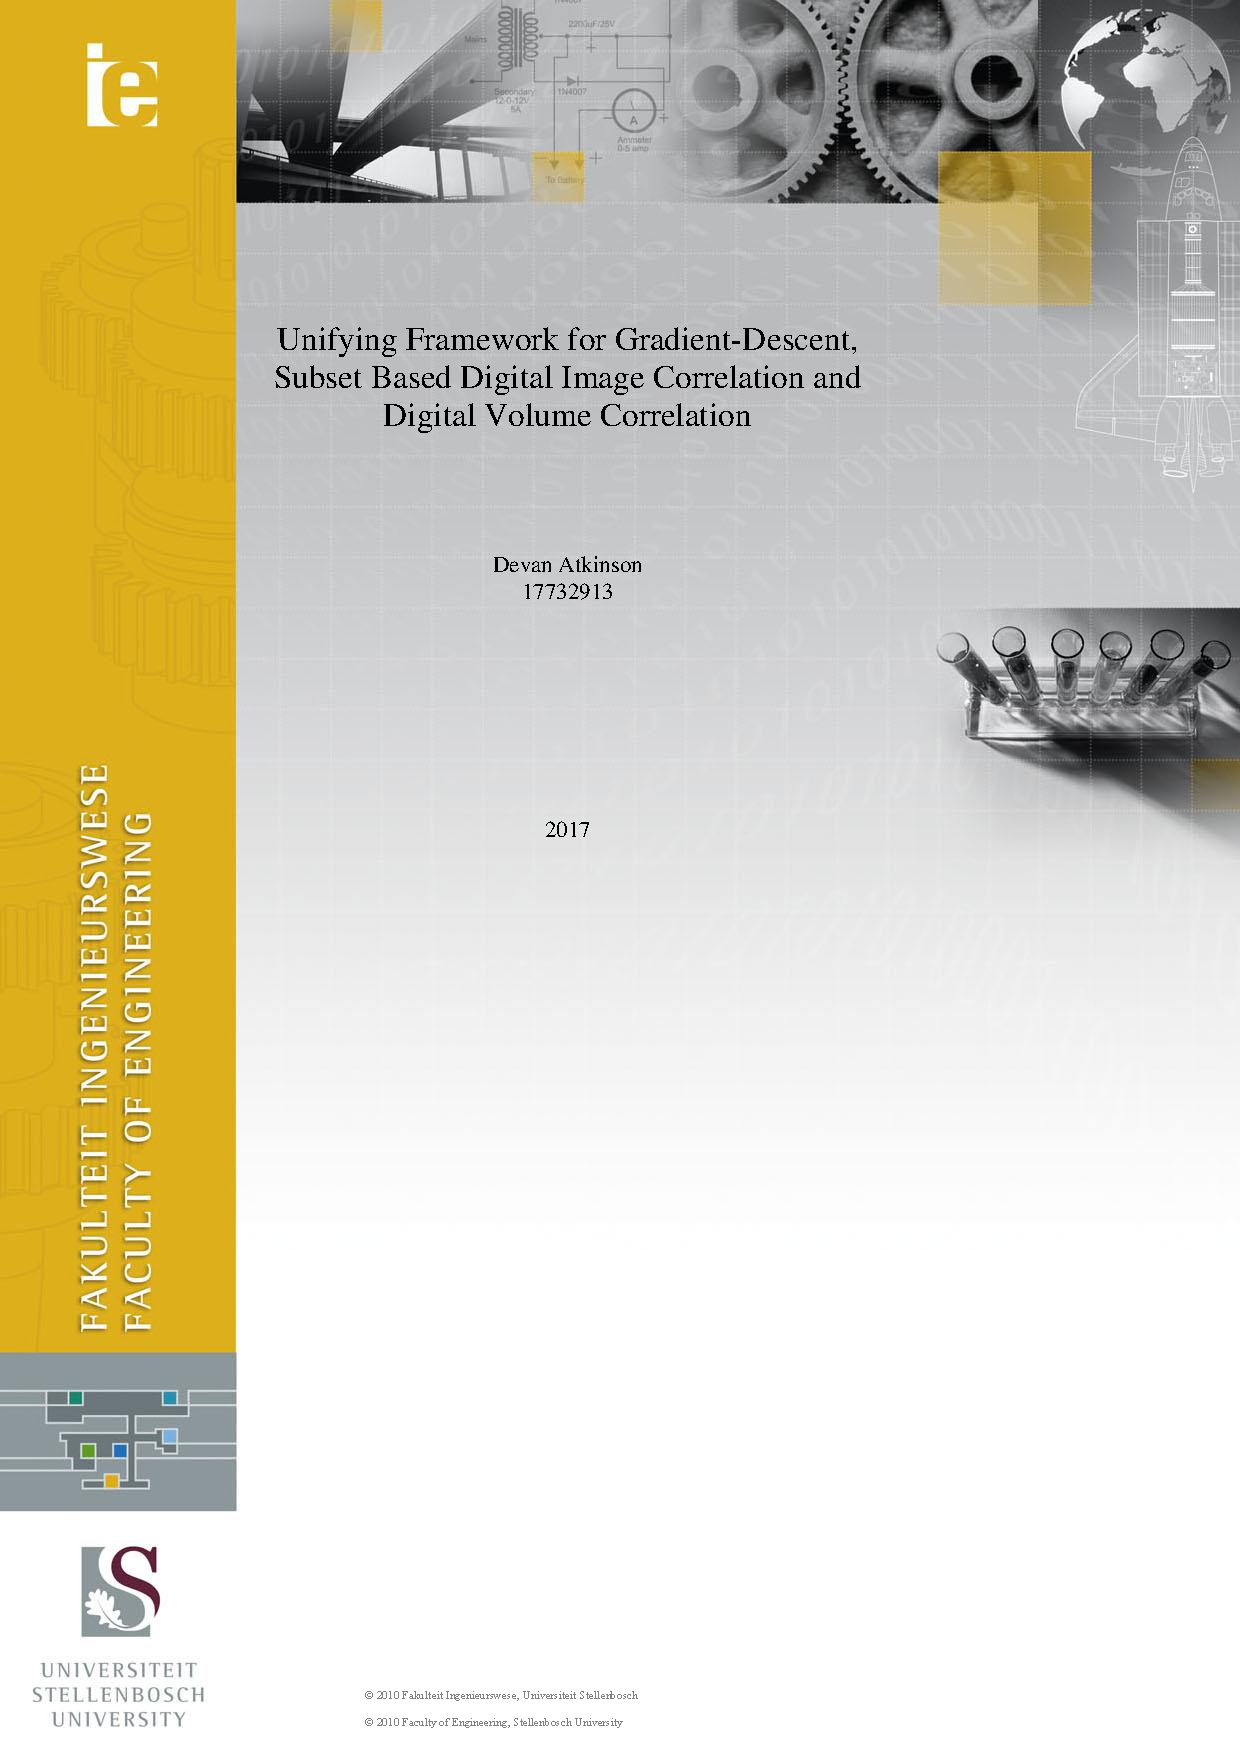
\includepdf{Cover.pdf}
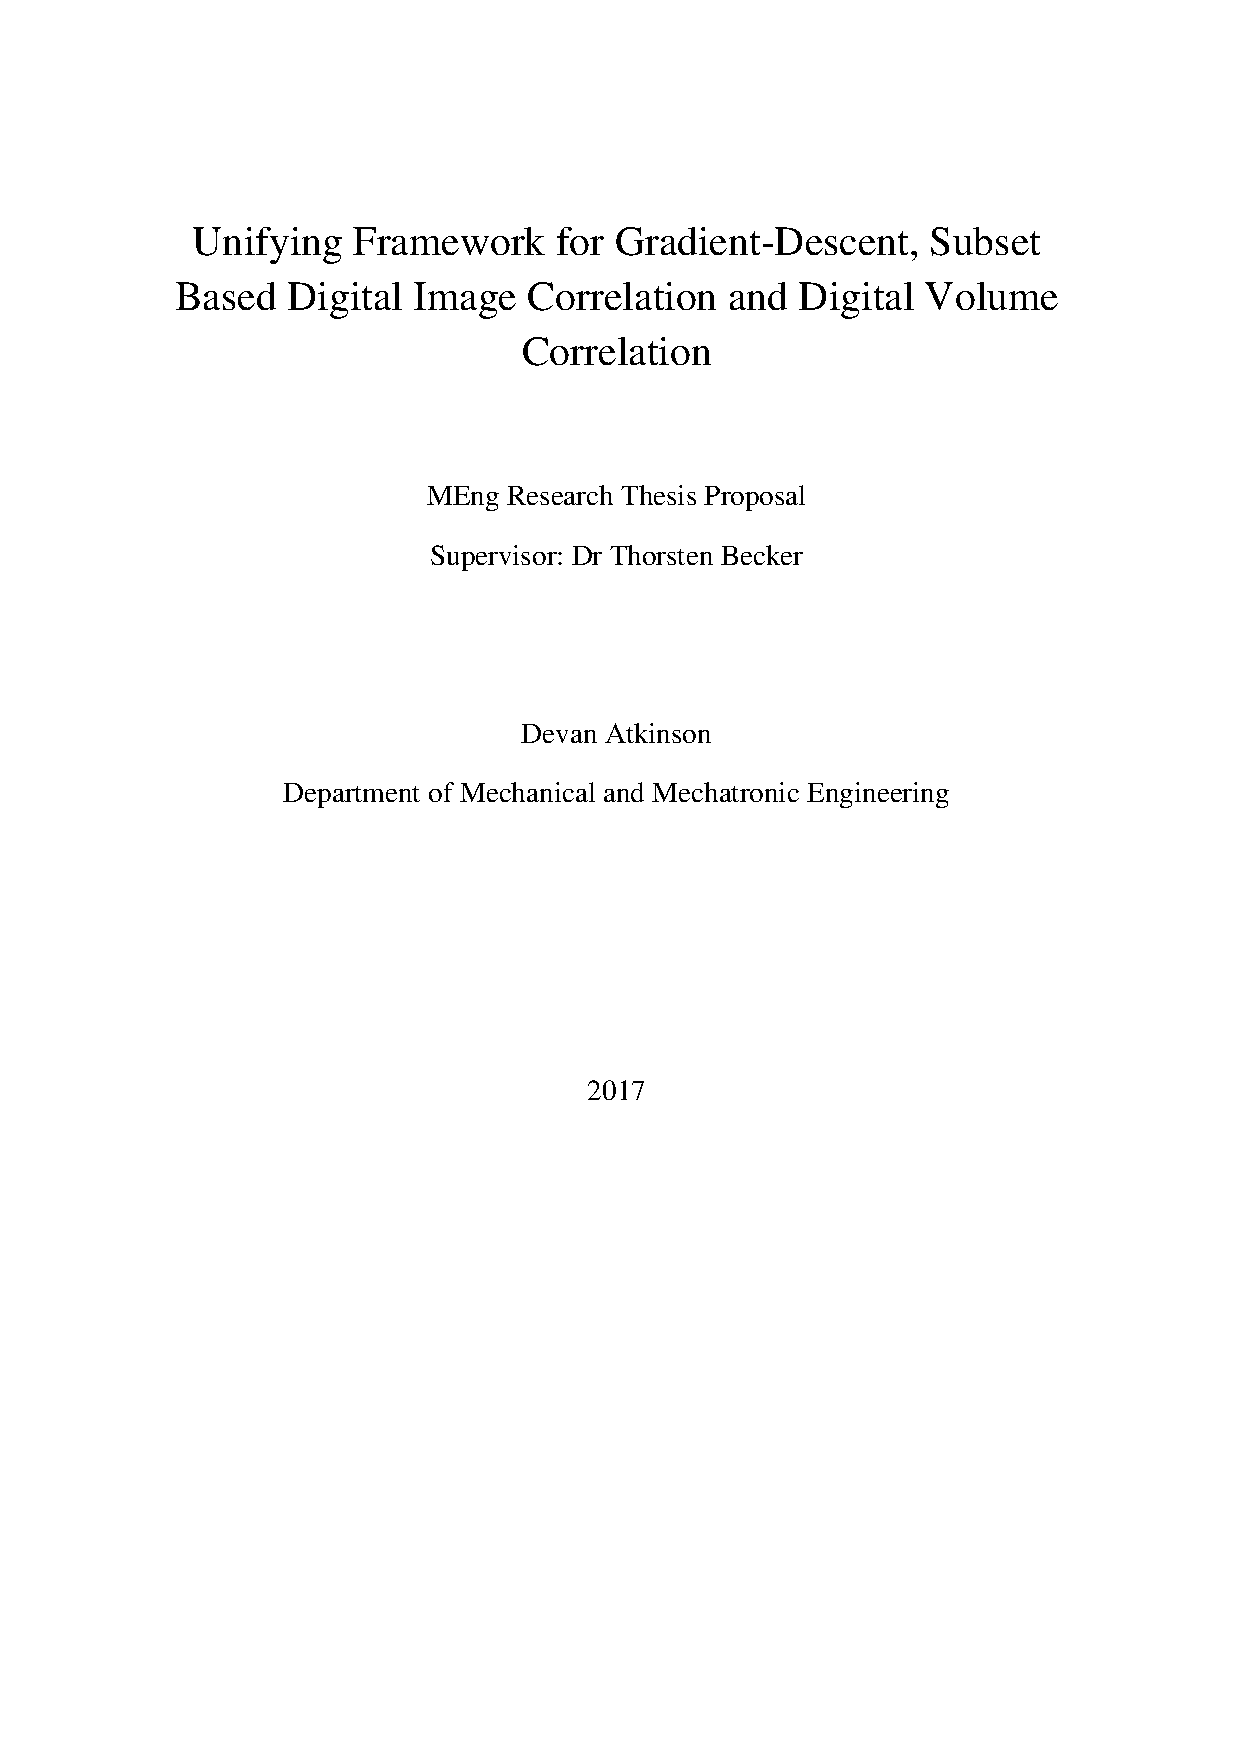
\includepdf{TitlePage.pdf}

\includepdf{plagiarism.pdf}
\chapter*{Abstract}
Digital Image Correlation (DIC) and Digital Volume Correlation (DVC) are becoming widely used tools, in the field of material science, to measure the displacements and deformations of specimens. However the high cost of commercial DIC and DVC software and the limited control offered over the correlation process in both commercial and open-source software limits its widespread adoption. This paper proposes a project which aims to create a Matlab based program capable of performing 2D DIC and DVC on a given set of images while allowing the user control over the correlation process. It is hypothesised that the different DIC algorithms use different methods to perform the same tasks in the correlation process. Thus by analysing these algorithms it is possible to combine these different methods into one program which will allow the user to select which methods to use for the various correlation tasks. If successful, this project will produce a freely available program, which offers many of the correlation methods of the different DIC algorithms, so that users will be able to perform in depth DIC and DVC analyses.

% which allows users full control over the correlation process 

% This project primarily consists of researching different DIC algorithms to determine the various methods of performing correlation and incorporating these methods into the program so that the user can choose which to use.



%  This project is motivated by the lack of freely available DIC software which allows the user to control the correlation process. This software is intended to combine most of the 2D DIC algorithms that are beneficial to material science applications into a single code. The successful completion of this project  will allow researchers of material science a comprehensive tool to determine specimen deformation from images taken of the specimen.

\tableofcontents
\listoffigures
\chapter{Introduction}

\chapter{Calibration}
\section{Calibration}
Calibration is a necessary process that must be completed in order to extract metric information from images. The calibration process solves for parameters that define the optical characteristics of the camera, parameters that define the orientation and position of the camera coordinate system to the world coordinate system and parameters that define the distortions that must be corrected in the images. 

The parameters that define the optical characteristics and the distortions are referred to as intrinsic parameters since they are fixed for a specific camera. The parameters that describe the orientation and position of the camera within the world coordinate system are extrinsic parameters because they change if the camera is moved. \todo{explain intrinsic and extrinsic better}

Multiple methods of calibration exist however calibration using a calibration plate is used in this project since it is one of the most popular methods and making a calibration plate is relatively simple and inexpensive. Calibration for distortion parameters will not be focused on in this section. \todo{take out distortion not used}

\subsection{Inverse problem}
Calibration is essentially a method of finding the parameters that allow 3D coordinates in the world coordinate system to be accurately related to 2D coordinates in the image coordinate system. Thus the inputs, 3D world coordinates, and outputs, 2D image coordinates, needed to be used to solve for the parameters which describe the relationship between the two which constitutes an inverse problem.

Inverse problems are typlically hard to solve and calibration is no exception. In order to solve for the calibration parameters more reliably the camera model that relates world points to sensor points is broken down to the simple pinhole camera model initially in order to solve for as few parameters as possible initially. These parameters are solved for using a closed form solution which gives good estimates to the parameters. Thereafter once these parameters have been estimated the camera model is made more complex by introducing radial distortion in order to account for imperfections in the lens system of the camera. These radial parameters are first estimated and once each parameter has a corresponding estimate all the parameters are optimized in an iterative manner.

This inverse problem is sensitive to errors in the 3D world coordinates (inputs) and 2D image coordinates (outputs) used. Thus these need to be known to a high degree of accuracy in order to solve for the intrinsic and extrinsic camera parameters reliably. This is achieved by using a calibration plate.

\subsection{Calibration plate}
A calibration plate is an object with a flat surface containing a high-contrast, regular pattern. The pattern is such that it contains definitive, point-like features which can be located to a high degree of accuracy within images taken of it. For example a checker board pattern allows for accurate calculation of the points at the corners of the squares. Thus the coordinates of these point-like features on the calibration plate will be known (inputs) and the coordinates of these point-like features in the image can be determined to a high degree of accuracy (outputs).

Since images inherently contain some level of noise it is best to have an overdetermined system of equations. This is accomplished by taking multiple images of the calibration plate and changing the relative position and orientation between the calibration plate and the camera for each image. This effectively reduces the effects of noise; making the system more robust.

\subsection{Homography}
\label{sec: homography}
Homography is a transformation that can be applied to points on a plane to bring it into alignment with another plane. It is used to bring the points on the calibration plate in the world coordinate system into alignment with their location in the image in the sensor coordinate system. The transformation from world coordinates to sensor coordinates in equation \ref{eq:world 2 sensor} is a type of homography.

Treating the calibration plate such that it lies in the x-y plane of the world coordinate system; the homography, $\bm{H}$, for calibration is given by the following equation.
\begin{equation}
  \begin{bmatrix}
  x_s \\
  y_s \\
  1
  \end{bmatrix} = 
  \alpha
  \begin{bmatrix}
  f_x & f_s & c_x & 0\\
  0 & f_y & c_y & 0\\
  0 & 0 & 1 & 0
  \end{bmatrix}
  \begin{bmatrix}
  r_{11} & r_{12} & r_{13} & t_1 \\
  r_{21} & r_{22} & r_{23} & t_2 \\
  r_{31} & r_{32} & r_{33} & t_3 \\
  0 & 0 & 0 & 1
  \end{bmatrix}
  \begin{bmatrix}
  x_w \\
  y_w \\
  0 \\
  1
  \end{bmatrix} \\
\end{equation}
This can be reduced to 
\begin{align}
  \begin{bmatrix}
  x_s \\
  y_s \\
  1
  \end{bmatrix} &=
  \alpha
  \begin{bmatrix}
  f_x & f_s & c_x \\
  0 & f_y & c_y \\
  0 & 0 & 1 
  \end{bmatrix}
  \begin{bmatrix}
  r_{11} & r_{12} & t_1 \\
  r_{21} & r_{22} & t_2 \\
  r_{31} & r_{32} & t_3 
  \end{bmatrix}
  \begin{bmatrix}
  x_w \\
  y_w \\
  1
  \end{bmatrix} \\
  &= \alpha \bm{K} 
  \begin{bmatrix}
  \bm{r}_1 & \bm{r}_2 & \bm{t}
  \end{bmatrix}
  \begin{bmatrix}
  x_w \\
  y_w \\
  1
  \end{bmatrix} \\
  &= \alpha
  \begin{bmatrix}
  h_1 & h_2 & h_3 \\
  h_4 & h_5 & h_6 \\
  h_7 & h_8 & h_9
  \end{bmatrix} 
  \begin{bmatrix}
  x_w \\
  y_w \\
  1
  \end{bmatrix}
  =\alpha \bm{H} 
  \begin{bmatrix}
  x_w \\
  y_w \\
  1
  \end{bmatrix} \label{eq: homography 1}
\end{align}
Here $\bm{r}_1$ and $\bm{r}_2$ are the first and second columns of the rotation matrix. It is clear that the homography matrix contains both intrinsic and extrinsic parameters and thus it is different for each image taken of the calibration plate. Additionally note that the homography matrix is defined up to a scale factor.

%http://www.learnopencv.com/homography-examples-using-opencv-python-c/

\subsection{Estimating homography with direct linear transform}
The homographies that relate the world coordinates of the calibration plate targets to the targets in the image can be estimated using direct linear transformation \cite{zhangtut}. Equation \ref{eq: homography 1} can be written out as
\begin{align}
  x_s &= \alpha \left( h_1 x_w + h_2 y_w + h_3 \right) \label{eq: homo line 1} \\
  y_s &= \alpha \left( h_4 x_w + h_5 y_w + h_6 \right) \label{eq: homo line 2} \\
  1 &= \alpha \left( h_7 x_w + h_8 y_w + h_9 \right) \label{eq: homo line 3}.
\end{align}
The scale factor, $\alpha$, can be eliminated by dividing equations \ref{eq: homo line 1} and \ref{eq: homo line 2} by \ref{eq: homo line 3} to get
\begin{align}
  x_s \left( h_7 x_w + h_8 y_w + h_9 \right) &= \left( h_1 x_w + h_2 y_w + h_3 \right) \\
  y_s \left( h_7 x_w + h_8 y_w + h_9 \right) &= \left( h_4 x_w + h_5 y_w + h_6 \right)
\end{align}
These equations then reduce to
\begin{align}
  - h_y x_w x_s - h_8 y_w x_s + h_1 x_w + h_2 y_w +h_3 &= h_9 x_s \label{eq: solve homo 1}\\
  - h_7 x_w y_s - h_8 y_w y_s + h_4 x_w + h_5 y_w + h_6 &= h_9 y_s. \label{eq: solve homo 2}
\end{align}
In order to avoid the trivial solution where every element in the homogrpahy matrix is equal to zero; constraints need to be placed on the elements of the homography matrix. In this case the element $h_9$ is set equal to 1 however other constraints are also possible such as $h_7^2 + h_8^2 + h_9^2 = 1$. Note that if the true value of $h_9$ is close to zero then this assumption will introduce a singluarity \cite{emerging}.

Each target, having points $x_{w_i}$ and $y_{w_i}$, on the calibration plate that is captured within an image of the calibration plate, having points $x_{s_i}$ and $y_{s_i}$, provides both an equation \ref{eq: solve homo 1} and \ref{eq: solve homo 2}. These are then combined into an equation of the form
\begin{align}
  \begin{bmatrix}
  x_{w_1} & y_{w_1} & 1 & 0 & 0 & 0 & -x_{w_1} x_{s_1} & -y_{w_1} x_{s_1} \\
  0 & 0 & 0 & x_{w_1} & y_{w_1} & 1 & -x_{w_1} y_{s_1} & -y_{w_1} y_{s_1} \\
  x_{w_2} & y_{w_2} & 1 & 0 & 0 & 0 & -x_{w_2} x_{s_2} & -y_{w_2} x_{s_2} \\
  0 & 0 & 0 & x_{w_2} & y_{w_2} & 1 & -x_{w_2} y_{s_2} & -y_{w_2} y_{s_2} \\
  \vdots & \vdots & \vdots & \vdots & \vdots & \vdots & \vdots & \vdots 
  \end{bmatrix}
  \begin{bmatrix}
  h_1 \\
  h_2 \\
  h_3 \\
  h_4 \\
  h_5 \\
  h_6 \\
  h_7 \\
  h_8
  \end{bmatrix} =
  \begin{bmatrix}
  x_{s_1} \\
  y_{s_1} \\
  x_{s_2} \\
  y_{s_2} \\
  \vdots
  \end{bmatrix}
\end{align}
This overdetermined system of equations then can be used to solve for the homography matrices of each calibration image using least squares. This is the first step involved in calibration. \todo{speak about normalisation}

\subsection{Absolute conic}
\label{sec: abs conic}
As mentioned before two objects that are parallel in Euclidean space appear to intersect each other in projective space. The intersection of these two lines in projective space occurs at a point that lies on the plane at infinity. If a point lies upon the plane at infinity its $w$ is equal to zero in homogeneous coordinates.

The absolute conic lies on the plane at infinity and is defined by the set of points, $\tilde{\bm{x}}_{ac} = [x, y, z, w]^T$, that satisfies the following. 
\begin{align}
  w = 0 \\
  \bm{x}_{ac}^T \bm{x}_{ac}=x^2 + y^2 + z^2 = 0 
  \label{eq:conditions of absolute conic}
\end{align}
Here tilde is used to indicate homogeneous coordinates whereas $\bm{x}_{ac} = [x, y, z]^T$ would be the point in Euclidean space.

Thus it is the conic of purely imaginary points that lies upon the plane at infinity. The importance of the absolute conic is that it is invariant under any Euclidean transformations. In other words the relative position of the absolute conic to a moving camera is unaffected by extrinsic parameters. Consider a point $\bm{x}_{ac}$ in Euclidean space in the world coordinate system that lies on the absolute conic. It has homogeneous coordinates $\tilde{\bm{x}}_{ac}=[\bm{x}_{ac}^T, 0]^T$ in projective space. Applying a different rotation and translation to this point to obtain $\tilde{\bm{x}}_{ac}'$, which is equivalent to moving the camera in the world coordinate system, a corresponding point is obtained in the camera coordinate system.
\begin{align}
  \tilde{\bm{x}}_{ac}' &=
  \begin{bmatrix}
  \bm{R} & \bm{T} \\
  \bm{0} & 1
  \end{bmatrix}
  \tilde{\bm{x}}_{ac} =
  \begin{bmatrix}
  r_{11} & r_{12} & r_{13} & t_1 \\
  r_{21} & r_{22} & r_{23} & t_2 \\
  r_{31} & r_{32} & r_{33} & t_3 \\
  0 & 0 & 0 & 1
  \end{bmatrix}
  \begin{bmatrix}
  x_{ac} \\
  y_{ac} \\
  z_{ac} \\
  0
  \end{bmatrix} \\
  &= 
  \begin{bmatrix}
  \bm{R} \bm{x}_{ac} \\
  0
  \end{bmatrix}
\end{align}
It is clear that this point still lies on the plane at infinity since its $w$ is equal to zero. More importantly it can be proven that this point $\bm{x}_{ac}'$ is on the same absolute conic.
\begin{equation}
  \bm{x}_{ac}'^T \bm{x}_{ac}' = \left( \bm{R} \bm{x}_{ac} \right) ^T \left( \bm{R} \bm{x}_{ac} \right) = \bm{x}_{ac}^T \bm{R}^T \bm{R} \bm{x}_{ac} = \bm{x}_{ac}^T \bm{x}_{ac} = 0
\end{equation}
Thus the absolute conic is invariant to Euclidean transformations. Now consider again a point, $\bm{x}_{ac}$, lying on the absolute conic. The corresponding point, $\bm{m}_s$, in the sensor plane is given by
\begin{align}
  \tilde{\bm{m}}_s &= \frac{1}{\alpha} \bm{K} 
  \begin{bmatrix}
  \bm{R} & \bm{T} \\
  \bm{0} & 1
  \end{bmatrix}
  \begin{bmatrix}
  \bm{x}_{ac} \\
  0
  \end{bmatrix} = \frac{1}{\alpha} \bm{K}
  \begin{bmatrix}
  \bm{R} \bm{x}_{ac} \\
  0
  \end{bmatrix} \\
  \therefore \bm{m}_s &= \frac{1}{\alpha} \bm{K} \bm{R} \bm{x}_{ac}.
\end{align}
Checking whether this point satisfies equation \ref{eq:conditions of absolute conic} results in
\begin{equation}
  \bm{m}_s^T \bm{K}^{-T} \bm{K}^{-1} \bm{m}_s = \frac{1}{\alpha^2} \bm{x}_{ac}^T \bm{R}^T \bm{R} \bm{x}_{ac} = \frac{1}{\alpha^2} \bm{x}_{ac}^T \bm{x}_{ac} = 0
\end{equation}
Thus the image of the absolute conic is itself an imaginary conic. The image of the absolute conic is defined by $\bm{K}^{-T} \bm{K}^{-1}$ \cite{luong1997self}. Thus since the image of the absolute conic is dependent only on intrinsic camera parameters it can be used to solve for the intrinsic camera parameters.

% http://www.cs.unc.edu/~marc/tutorial/node87.html
\subsection{Constraints on intrinsic parameters}
\label{sec: intrinsic constraints}
According to Zhang \cite{emerging} there are two constraints placed upon the intrinsic parameters of the camera. These are important later on in the solving for these intrinsic parameters. The plane of the calibration plate in the camera coordinate system is given by \cite{emerging} 
\begin{equation}
  \begin{bmatrix}
  \bm{r}_3 \\
  \bm{r}_3^T \bm{t}
  \end{bmatrix}^T
  \begin{bmatrix}
  x \\
  y \\
  z \\
  w
  \end{bmatrix} = 0.
\end{equation}
Here $w$ is zero for points on the plane at infinity and one for those that are not. This plane intersects the plane at infinity on a line and it happens that $[\bm{r}_1^T, 0]^T$ and $[\bm{r}_2^T, 0]^T$ are points on this line \cite{emerging}. Thus it is known that any point on this line, $x_c^{\infty}$, is a linear combination of these two points.
\begin{equation}
  x_c^{\infty} = a \begin{bmatrix}
  \bm{r}_1 \\
  0
  \end{bmatrix} + b
  \begin{bmatrix}
  \bm{r}_2 \\
  0
  \end{bmatrix} =
  \begin{bmatrix}
  a \bm{r}_1 + b \bm{r}_2 \\
  0
  \end{bmatrix}
\end{equation}
Now assume that this point, $x_c^{\infty}$, lies on the absolute conic. Then this point must satisfy equation \ref{eq:conditions of absolute conic}. This would require that $a^2+b^2=0$ which results in the solution $b=\pm a i$, where $i=\sqrt{-1}$. As a result it can be seen that the two points along this line intersect the absolute conic at
\begin{equation}
  x_c^{\infty} = a 
  \begin{bmatrix}
  \bm{r}_1 \pm i \bm{r_2} \\
  0
  \end{bmatrix}.
\end{equation}
Since these points lie on the absolute conic they are invariant under Euclidean transformations. Their projection, up to a scale factor, in the sensor coordinate system is given by
\begin{equation}
  x_s^{\infty} = \bm{K} \left( \bm{r}_1 \pm \bm{r}_2 \right) = \bm{h}_1 \pm i \bm{h}_2.
\end{equation}
Substituting these points into equation \ref{eq:conditions of absolute conic} results in
\begin{equation}
  \left( \bm{h}_1 \pm i \bm{h}_2 \right)^T \bm{K}^{-T} \bm{K}^{-1} \left( \bm{h}_1 \pm i \bm{h}_2 \right) = 0.
\end{equation}
Requiring both the imaginary and real parts of this equation to equal zero results in two constraints on the intrinsic camera parameters.
\begin{align}
\label{eq:intrinsic constraints}
  \bm{h}_1^T \bm{K}^{-T} \bm{K}^{-1} \bm{h}_2 &= 0 \\
  \bm{h}_1^T \bm{K}^{-T} \bm{K}^{-1} \bm{h}_1 &= \bm{h}_2^T \bm{K}^{-T} \bm{K}^{-1} \bm{h}_2
\end{align}

\subsection{Intrinsic parameters and the absolute conic}
\label{sec: parameters and the absolute conic}
An homography, $\bm{H}$, between the calibration plate and the image of the calibration plate can be estimated. This homography can then be used to solve for the image of the absolute conic. Once the image of the absolute conic is known it can be used to solve for the intrinsic camera parameters. The image of the absolute conic can be represented as
\begin{equation}
  \bm{B} = \bm{K}^{-T} \bm{K}^{-1} = 
  \begin{bmatrix}
  b_{11} & b_{12} & b_{13}\\
  b_{12} & b_{22} & b_{23} \\
  b_{13} & b_{23} & b_{33}
  \end{bmatrix}
\end{equation}
Since $\bm{B}$ is symmetric its contents can be represented by a 6D vector $\bm{b}=[b_{11} b_{12} b_{22} b_{13} b_{23} b_{33}]^T$. Let $\bm{h}_i = [h_{i1} h_{i2} h_{i3}]^T$ to be the i\textsuperscript{th} column of $\bm{H}$. Then
\begin{equation}
  \bm{h}_I^T \bm{B} \bm{h}_j = \bm{v}_{ij} \bm{b}
\end{equation}
where 
\begin{equation}
  \bm{v}_{ij} = [ h_{i1} h_{j1}, h_{i1} h_{j2} + h_{i2} h_{j1}, h_{i2} h_{j2}, h_{i3} h_{j1} + h_{i1} h_{j3}, h_{i3} h_{j2} + h_{i2} h_{j3}, h_{i3} h_{j3}]^T.
\end{equation}
Then equation \ref{eq:intrinsic constraints} can be rewritten as 
\begin{equation}
  \begin{bmatrix} 
  \bm{v}_{12}^T \\
  ( \bm{v}_{11} - \bm{v}_{22})^T
  \end{bmatrix} \bm{b} = \bm{0}
\end{equation}
A separate version of this equation exist for each image taken of the calibration plate and these equations can be stacked, in $\bm{V}$, to give
\begin{equation}
  \bm{V}\bm{b}=\bm{0}.
\end{equation}
The solution for $\bm{b}$, up to a scale factor $\lambda$, is known to be the eigenvector of $\bm{V}^T\bm{V}$ associated with the smallest eigenvalue \cite{emerging}. Once b has been determined it can be used to determine the intrinsic parameters of matrix $\bm{K}$. The relation between $\bm{B}$ and $\bm{K}$ is $\bm{B}=\lambda \bm{K}^{-T} \bm{K}^{-1}$. The intrinsic parameters are determined as follows.
\begin{align}
  c_y &= (b_{12} b_{13} - b_{11} b_{23})/(b_{11} b_{22} - b_{12}^2) \\
  \lambda &= b_{33} -(b_{13}^2 + c_y(b_{12} b_{13} - b_{11} b_{23}))/b_{11}\\
  f_x &= \sqrt{\frac{\lambda}{b_{11}}} \\
  f_y &= \sqrt{\frac{\lambda b_{11}}{b_{11} b_{22} - b_{12}^2}} \\
  f_s &= \frac{-b_{12} f_x^2 f_y}{\lambda} \\
  c_x &= \frac{f_s c_y}{f_y} - \frac{b_{13} f_x^2}{\lambda}
\end{align}
Thereafter the extrinsic parameters can be determined.
\begin{align}
  \bm{r}_1 &= \lambda \bm{K}^{-1} \bm{h}_1 \\
  \bm{r}_2 &= \lambda \bm{K}^{-1} \bm{h}_2 \\
  \bm{r}_3 &= \bm{r}_1 \times \bm{r}_2 \\
  \bm{T} &= \lambda \bm{K}^{-1} \bm{h}_3
\end{align}
At this point it is necessary to incorporate distortions and use them to find better approximations for the intrinsic and extrinsic parameters.

\todo{this section is too close to the paper} %a fleixible new technique and reading 1
% by which the optical characteristics of a camera and the relation between its coordinate system and the world coordinate system are determined. It is performed in order to be able to extract \hl{metric} information from images accurately.

\subsection{Closed form solution}
Sections \ref{sec: homography} throught to \ref{sec: parameters and the absolute conic} illustrate that estimates to the intrinsic and extrinsic parameters can be obtained by first determining the homographies for each calibration image, then these can be used to determine the image of the abolute conic which in turn can be used to determine the intrinsic and extrinsic camera parameters. This is closed form solution is the first part of the calibration process

put inverse problem in calibration plate section

explain homography and absolute conic

then explain closed form solution and optimization - give closed form and explain optimization


\subsection{Distortion in Calibration}
The closed form solution given above does not take distortion into account since it is based on the pinhole camera model. It is only once the closed form solution to the extrinsic and intrinsic parameters is optimised that distortion can be accounted for during the calibration process. As already presented, there are many types of distortion that occur when an image is taken. However it is seldom possible to take all of these distortion types into account since the more distortion paramters introduced into the camera model; the more likely the optimization process becomes unstable.

It has been found \todo{add reference for this} that good calibration results can be achieved by taking only radial distortion into accound during calibration \cite{tsai1987versatile,wei1994implicit}. This is beneficial since it is possible to solve for initial guesses to the radial distortion parameters which helps the optimisation process to avoid local minima as a result of the distortion parameters used.

The distortion applied to the points on the image plane is of the form
\begin{align}
  \begin{bmatrix}
  x_{i_{distorted}} \\
  y_{i_{distorted}}
  \end{bmatrix} &=
  1 + k_1 r^2 + k_2 r^4
  \begin{bmatrix}
  x_i \\
  y_i
  \end{bmatrix}\\
  \text{where} \quad \quad r &= \sqrt{x_i^2 + y_i^2}.
\end{align}

At this point the intrinsic and extrinsic parameters have been determined using the pinhole camera model and the error between the predicted calibration plate targets and the actual location of these in the images is attributed to radial distortion \cite{zhangtut}. This error is represented as
\begin{equation}
  d_1 = x_{s_{actual}} - x_{s_{calculated}}
\end{equation}

An undistorted point, $x_i$ is distorted to point $\tilde{x_i}$ according to
\begin{align}
  \tilde{x_i} &= u_c + (x_i-u_c)*(1 + k1 r^2 + k2 r^4) \\
  &= u_c + x_i - u_c + (x_i-u_c)*(1 + k1 r^2 + k2 r^4) \\
  &= x_i + (x_i-u_c)*(1 + k1 r^2 + k2 r^4) \\
  &= x_i + d_{2_i}
\end{align}

The distortion parameters can be estimated by minimizing the difference between $d_1$ and $d_2$. Thus the least squares solution to the overdetermined system is what is needed.

\chapter{Correlation}
The Lucas-Kanade algorithm was used in combination with the zero-mean normalised sum of squared differences correlation criteria. This correlation criteria was chosen since it takes into account offset and scaling in the light intensities of the images making the overall algorithm more robust. The Lucas-Kanade algorithm assumes that the deformation of the image is constant over a area of the image referred to as the subset. As such this algorithm tries to find the deformation field that best corrects a subset of the deformed image so that it appears to be the same as the reference image. 

\section{Correlation criteria}
% Each correlation criteria is based off of a cost function which is usually a variation of the
% sum of squared differences between the intensities of the reference and investigated subset.
% They vary in the scaling and offset that is applied to the investigated subset’s intensity
% values.


A correlation criteria is a mathematical way of quantifying how well a subset in one image matches to a subset in another image. It is used to determine whether the deformation field that has been solved for is sufficiently accurate to explain how the deformed image is related to the reference image. As such it is important that the correlation criteria reliably indicates the fit between the two subsets.

The zero-mean normalised sum of squared differences (ZNSSD) correlation criteria is one of the most robust options for a correlation criteria since it accounts for both lighting offset and scaling between the reference and deformed images. Correlation criteria are based off of a cost function which is usually a variation of the sum of squared difference between the pixel values of a subset of the reference image and a subset of the deformed image. The ZNSSD correlation criteria has the following cost function.
\begin{equation}
\label{eq:cf znssd}
  \chi_{ZNSSD}^2 = \sum_i \left( a G_i + b - F_i \right) ^2
\end{equation}
The offset $b$ and scaling $a$ can be solved for by treating it as an additional parameter of the optimisation problem. However it is preferred to determine the optimal estimates for $b$ and $a$ by taking the derivative of the cost function with respect to $a$ and $b$ separately and setting this to zero.
\begin{align}
  \frac{\partial \chi_{ZNSSD}^2 }{\partial a} &= 2 \sum_i \left( a_{opt} G_i + b- F_i \right) G_i = 0\\
  \Rightarrow a_{opt} &= \frac{\sum_i \left( F_i - b \right) G_i}{\sum_i G_i^2} \\
  \frac{\partial \chi_{ZNSSD}^2 }{\partial b} &= 2 \sum_i \left( a G_i + b_{opt} - F_i \right) = 0\\
  \Rightarrow b_{opt} &= \frac{\sum_i F_i -a G_i}{n}
\end{align}
Here $n$ is the number of pixels in the subset and $\mean{F}$ and $\mean{G}$  are the average intensity values for the reference and investigated subset respectively. These can be solved to obtain
\begin{align}
  a_{opt} &= \frac{\sum_i \mean{F_i} \mean{G_i}}{\sum_i \mean{G_i^2}}, &b_{opt}&= \mean{F} -\mean{G} \frac{\sum_i \mean{F_i} \mean{G_i}}{\sum_i \mean{G_i^2}} \\
  \text{where} \quad \quad \mean{F_i} &= F_i - \mean{F} \quad \quad \quad \quad \text{and} & \mean{G_i} &= G_i -\mean{G}
\end{align}
Substituting these into equation \ref{eq:cf znssd} results in the correlation criteria.
\begin{equation}
  \chi_{ZNSSD}^2 = \sum_i \left( \left( \frac{\sum_i \mean{F_i} \mean{G_i}}{\sum_i \mean{G_i^2}} G_i - \mean{G} \frac{\sum_i \mean{F_i} \mean{G_i}}{\sum_i \mean{G_i^2}} \right) - F_i + \mean{F} \right) ^2
\end{equation} 



\section{Warp function}
When applying DIC to to material science the deformation behaviour of materials under load must be taken into account. This is because the deformation of the material causes the speckle pattern on its surface to deform in the same way. This is an issue since the pattern contained within a subset of the reference image will be deformed in the second image which can cause difficulties in matching the two subsets.

This is solved by allowing for the subsets to deform in a similar way to that of the material by defining the allowable deformations in a warp function. The purpose of these warp functions is to transform the pixel coordinates of the reference subset so that the resulting pattern is closer to the pattern in the deformed image. For this analysis the common warp function which accounts for affine transformations is used since it is consistent with the strains that the material is expected to experience. Thus by determining the warp function parameters for a specific subset; the strains for that subset are also determined.
\begin{equation}
  W (\bm{\zeta},\bm{p}) = 
  \begin{bmatrix}
  \Delta x_{warp} \\
  \Delta y_{warp}
  \end{bmatrix} 
  = \begin{bmatrix}
  1+\frac{\partial u}{\partial x} & \frac{\partial u}{\partial y} & u\\
  \frac{\partial v}{\partial x} & 1+\frac{\partial v}{\partial y} & v \\
  0 & 0 & 1
  \end{bmatrix}
  \begin{bmatrix}
  \Delta x \\
  \Delta y \\
  1
  \end{bmatrix}.
  \label{eq:warp}
\end{equation}
Here $u$ and $v$ represent the displacements in the x and y directions respectively, $\frac{\partial u}{\partial x}$ and $\frac{\partial v}{\partial y}$ represent the elongation in the x and y directions respectively whereas $\frac{\partial v}{\partial x}$ and $\frac{\partial u}{\partial y}$ represent the shear deformation of the subset. All of these variables that explain how the subset is warped and translated are stored within the vector $\bm{p} = \begin{bmatrix} u & \frac{\partial u}{\partial x} & \frac{\partial u}{\partial y} & v & \frac{\partial v}{\partial x} & \frac{\partial v}{\partial y} \end{bmatrix}$ which are referred to as the warp function parameters. Additionally $\Delta x$ and $\Delta y$ are the distances from the centre of the undeformed subset to the pixel under consideration and are contained within the variable $\bm{\zeta} = \begin{bmatrix} \Delta x & \Delta y & 1 \end{bmatrix}^T$. The outputs $\Delta x_{warp}$ and $\Delta y_{warp}$ are the modified distances from the centre of the subset to the pixel under consideration. Thus it is the pixel locations within the subset that are modified in order to induce warp and not the subset itself which is warped by this function. In other words the $\Delta x$ and $\Delta y$ are warped by the function which has the effect of warping the subset itself since it changes the locations within the subset that are to be evaluated. Thus the warp function applied to a subset is mathematically expressed as
\begin{equation}
  F_{warped}=F(\bm{x_0}+W(\bm{\zeta},\bm{p}))
  \label{eq:subset warp}
\end{equation}
where $\bm{x_0} = \begin{bmatrix} x_0 & y_0 \end{bmatrix}^T$ are the x and y coordinates, in units of pixels, of the centre of the subset.

With most subset based DIC algorithms the more complex the warp function becomes the more computationally expensive each iteration is. This is because the correlation criteria must be optimized in terms of more variables leading to more work. \todo{keep this?}

\section{Interpolation}
It is clear that warping a subset according to equation \ref{eq:subset warp} requires that the light intensity values between pixel locations can be determined. This is an issue because images store this information in a discrete manner. This is solved by using interpolation to determine the light intensity values between pixels based on the light intensity values of neighbouring pixels. For the purposes of this project Matlab's built in interp2 fucntion was used to perform linear interpolation to determine the light intensity values for non-standard pixel locations where needed.


% For DIC to be useful in the field of material science it must be able to determine displacements to sub-pixel accuracy. This requires knowing the light intensity values, within an image, between pixel locations. This is an issue because images store this information in a discrete manner. Interpolation is used to determine the light intensity values between pixels based on the light intensity values of neighbouring pixels. For the purposes of this project Matlab's built in interp2 fucntion was used to perform linear interpolation to determine the light intensity values for non-standard pixel locations where needed.

\section{Subset matching}
The purpose of DIC is to find the warp function parameters which optimise the correlation criteria between a specific subset, $F$, in the reference image and the investigated subset, $G$, in the deformed image.\todo{check}. Multiple methods of doing this have been proposed; each with their own advantages and disadvantages. The Lucas-Kanade method is used in this project and it is explained here for the case of correlating a reference subset $F$ to the subset under investigation $G$.

The Lucas-Kanade method is one of the most widely used subset based DIC techniques. It makes use of intensity gradients to guide the search direction to optimise the correlation criteria. A limitation of the method is that it requires the displacement between the images to be small which is common in material science applications.

The Lucas-Kanade method can be implemented in two distinct ways that differ in correlation criteria function. The first, the original way, is referred to as the forward additive method which applies the current estimate of the warp function and the iterative improvement to the warp function parameters to the investigated subset to deform it in an attempt to obtain a subset closer to the reference subset. This deformed subset is then compared with the reference subset and the difference between the two is used to incrementally improve the warp function parameter estimates. In this method the Hessian matrix is dependent on the investigated subset's light intensity values, $G$, and as such it needs to be computed for each iteration of the solver.

The second method, the inverse compositional method, is a modification to the forward additive method in an effort to decrease the computational cost per iteration. For this method the current estimate for the warp function parameters, $\bm{p}$, is applied to the investigated subset while the iterative improvement to the warp function parameters, $\bm{\Delta p}$, is applied to the reference subset. This is done so that the Hessian that needs to be determined depends only on the reference subset and is independent of the warp function parameters which allows it to be pre-computed outside of the iterations. As a result this method is more efficient which means it takes less time to converge to the solution.

The algorithm explained here is based on the one proposed by B. Pan \cite{panfast}. It is the inverse compositional Lucas-Kanade method using the Guass-Newton approximation to the Hessian matrix. The algorithm used to solve for the optimal parameters of the warp function is derived from the correlation criteria used as given below.
\begin{equation}
  \chi_{ZNSSD}^2 = \sum_{\zeta}  \left[ \frac{F(\bm{x_0}+W(\zeta,\Delta \bm{p}))-\mean{F}}{\Delta F} -\frac{G(\bm{x_0}+W(\zeta,\bm{p}))-\mean{G}}{\Delta G}\right]^2
  \label{eq:correlation criteria solver}
\end{equation}
Notice that the current approximation for the warp function parameters, $\bm{p}$, is applied to the investigated subset while the iterative improvement to the warp function parameters, $\Delta \bm{p}$, is applied to the reference subset. Taking the first-order Taylor expansion of equation \ref{eq:correlation criteria solver} in terms of $\Delta \bm{p}$ gives
\begin{equation}
  \chi_{ZNSSD}^2 = \sum_{\zeta}  \left[ \frac{F(\bm{x_0}+\zeta)+\triangledown F \frac{\partial W}{\partial \bm{p}} \Delta\bm{p}-\mean{F}}{\Delta F} -\frac{G(\bm{x_0}+W(\zeta,\bm{p}))-\mean{G}}{\Delta G}\right]^2
\end{equation}
where $\triangledown F = \begin{bmatrix} \frac{\partial F(\bm{x_0} + \bm{\zeta})}{\partial x} & \frac{\partial F(\bm{x_0} + \bm{\zeta})}{\partial y} \end{bmatrix}$ is the gradients of the reference subset in the x and y directions and $\frac{\partial W}{\partial \bm{p}} = \begin{bmatrix} 1 & \Delta x & \Delta y & 0 & 0 & 0 \\ 0 & 0 & 0 & 1 & \Delta x & \Delta y \end{bmatrix}$ is the Jacobian of the warp function.

Taking the derivative of equation \ref{eq:correlation criteria solver} with respect to $\Delta \bm{p}$ and setting it to zero gives the least squares solution for finding $\Delta \bm{p}$.
% \begin{align}
%   \frac{\partial \chi_{ZNSSD}^2}{\partial \Delta \bm{p}} = 0 = 2 \sum_{\zeta}  \left[ \frac{F(\bm{x_0}+\zeta)+\triangledown F \frac{\partial W}{\partial \bm{p}} \Delta\bm{p}-\mean{F}}{\Delta F} -\frac{G(\bm{x_0}+W(\zeta,\bm{p}))-\mean{G}}{\Delta G}\right] \frac{\triangledown F \frac{\partial W}{\partial \bm{p}}}{\Delta F}\\
%   \Delta \bm{p} = - \sum_{\zeta} \left[ (\triangledown F \frac{\partial W}{\partial \bm{p}})^T (\triangledown F \frac{\partial W}{\partial \bm{p}}) \right]^{-1} \times \sum_{\zeta} \left[ (\triangledown F \frac{\partial W}{\partial \bm{p}})^T \times \left[ (F(\bm{x_0} + \bm{\zeta}) - \mean{F}) - \frac{\Delta F}{\Delta G}(G(\bm{x_0}+W(\bm{\zeta}, \bm{p}))-\mean{G}) \right] \right]\\
%   \Delta \bm{p} = - H^{-1} \times \sum_{\zeta} \left[ (\triangledown F \frac{\partial W}{\partial \bm{p}})^T \times \left[ (F(\bm{x_0} + \bm{\zeta}) - \mean{F}) - \frac{\Delta F}{\Delta G}(G(\bm{x_0}+W(\bm{\zeta}, \bm{p}))-\mean{G}) \right] \right]
% \end{align}

\begin{align}
  \frac{\partial \chi_{ZNSSD}^2}{\partial \Delta \bm{p}} &= 0 = 2 \sum_{\zeta}  \left[ \frac{F(\bm{x_0}+\zeta)+\triangledown F \frac{\partial W}{\partial \bm{p}} \Delta\bm{p}-\mean{F}}{\Delta F} -\frac{G(\bm{x_0}+W(\zeta,\bm{p}))-\mean{G}}{\Delta G}\right] \frac{\triangledown F \frac{\partial W}{\partial \bm{p}}}{\Delta F}\\
  \Delta \bm{p} &= - H^{-1} \times \sum_{\zeta} \left[ (\triangledown F \frac{\partial W}{\partial \bm{p}})^T \times \left[ (F(\bm{x_0} + \bm{\zeta}) - \mean{F}) - \frac{\Delta F}{\Delta G}(G(\bm{x_0}+W(\bm{\zeta}, \bm{p}))-\mean{G}) \right] \right]
  \label{eq:delta p} \\
  \text{where} \qquad H &= \sum_{\zeta} \left[ (\triangledown F \frac{\partial W}{\partial \bm{p}})^T (\triangledown F \frac{\partial W}{\partial \bm{p}}) \right]
\end{align}

Here $H$ is the Hessian matrix which remains constant since it depends only on the reference subset. Thus the Hessian matrix can be computed before the algorithm starts iterating in order to reduce computational costs. However in order to achieve this reduced computational cost the iterative improvement to the warp function parameters was applied to the reference subset. This means that the iterative improvement cannot simply be added to the old warp function parameters to obtain the updated warp function parameters. Instead the updated warp function parameters must be determined using the following equation.
\begin{align}
  W(\bm{\zeta},\bm{p_{new}})&=W(\bm{\zeta},\bm{p_{current}})\times W(\bm{\zeta},\Delta \bm{p})^{-1}\\
  &=\begin{bmatrix}
  1+\frac{\partial u}{\partial x} & \frac{\partial u}{\partial y} & u\\
  \frac{\partial v}{\partial x} & 1+\frac{\partial v}{\partial y} & v \\
  0 & 0 & 1
  \end{bmatrix}
  \begin{bmatrix}
  1+\Delta \frac{\partial u}{\partial x} & \Delta \frac{\partial u}{\partial y} & \Delta u\\
  \Delta \frac{\partial v}{\partial x} & 1+\Delta \frac{\partial v}{\partial y} & \Delta v \\
  0 & 0 & 1
  \end{bmatrix}^{-1}
  \label{eq:get new p}
\end{align}
The new approximation to the warp function parameters can then be extracted from this warp function matrix $W(\bm{\zeta},\bm{p_{new}})$.

\section{Algorithm outline}
The steps performed within the algorithm in order to achieve correlation are listed here in order to illustrate how the theory presented here is related to the code.

\begin{enumerate}
  \item First $\mean{F}$ is determined for the reference subset.
  \item Then $\triangledown F$ is calculated using Matlab's built in image gradient function (imgradientxy) and the Jacobian of the warp function is calculated. These are then used to determine the Hessian matrix.
  \item Thereafter $\Delta F$ is determined since it too remains constant.
  \item The initial guess for the warp function parameters is then used to calculate the $\Delta x_{warp}$ and $\Delta y_{warp}$ for the investigated subset $G$ using equation \ref{eq:warp}.
  \item $\Delta x_{warp}$ and $\Delta y_{warp}$ are used in equation \ref{eq:subset warp} to obtain the warped version of the investigated subset.
  \item $\mean{G}$ and $\Delta G$ are then determined.
  \item With all the necessary values determined; equation \ref{eq:delta p} can be used to calculate $\Delta \bm{p}$.
  \item Then equation \ref{eq:get new p} is used to determine the updated approximation to the warp function parameters.
  \item Step 4 until step 8 are repeated until convergence or until the warp function parameters are considered good enough.
\end{enumerate}


% The warp function parameters, $p$, are iteratively improved to obtain a better correlation criteria value by a method of non-linear optimization similar to that of Newton's method. 
% \begin{equation}
%   p^{k+1} = p^k + \Delta p
% \end{equation}
% The equation for $\Delta p$ is dependent on the warp function, the correlation criteria and the gradient descent approximation used. For illustration purposes the method will be derived using the sum of squared difference correlation criteria, with the warp function given in equation \ref{eq:warp} and Guass-Newton gradient descent approximation \cite{lucasUnifying}. Thus the correlation criteria to be minimized is 
% \begin{equation}
%   \chi^2= \sum_{\bm{x}} \left( G(W(\bm{x},\bm{p} + \Delta \bm{p})) - F(\bm{x})  \right) ^2.
% \end{equation}
% Taking the Taylor expansion of $G(W(\bm{x},\bm{p} + \Delta \bm{p}))$, this equation reduces to
% \begin{align}
%   \label{eq:lucas chi}
%   && \chi^2 &= \sum_{\bm{x}} \left( G(W(\bm{x},\bm{p})) +\nabla G \frac{\partial W(\bm{x},\bm{p})}{\partial \bm{p}} \Delta \bm{p} - F(\bm{x})  \right) ^2 &\\
%   \text{where}
%   &&\nabla G &= 
%   \begin{bmatrix}
%   \frac{\partial G(W(\bm{x},\bm{p}))}{\partial x} & \frac{\partial G(W(\bm{x},\bm{p}))}{\partial y}
%   \end{bmatrix} &\\
%   \text{and} &&\frac{\partial W(\bm{x},\bm{p})}{\partial \bm{p}} &= 
%   \begin{bmatrix}
%   \frac{\partial x_w}{\partial u} & \frac{\partial x_w}{\partial v} & \frac{\partial x_w}{\frac{\partial u}{\partial x}} & \frac{\partial x_w}{\frac{\partial u}{\partial y}} & \frac{\partial x_w}{\frac{\partial v}{\partial x}} & \frac{\partial x_w}{\frac{\partial v}{\partial y}} \\
%   \frac{\partial y_w}{\partial u} & \frac{\partial y_w}{\partial v} & \frac{\partial y_w}{\frac{\partial u}{\partial x}} & \frac{\partial y_w}{\frac{\partial u}{\partial y}} & \frac{\partial y_w}{\frac{\partial v}{\partial x}} & \frac{\partial y_w}{\frac{\partial v}{\partial y}}
%   \end{bmatrix} =
%   \begin{bmatrix}
%   1 & 0 & \Delta x & \Delta y & 0 & 0\\
%   0 & 1 & 0 & 0 & \Delta x & \Delta y
%   \end{bmatrix}\text{.}
% \end{align}
% Here $\nabla G$ is the gradient of the investigated subsets intensity calculated along its own coordinate frame but it is evaluated at the position given by the warp function. The optimal $\Delta \bm{p}$ can be found by taking the derivative of equation \ref{eq:lucas chi} with respect to $\Delta \bm{p}$ and setting it equal to zero.

% \begin{flalign}
%   && \frac{\partial \chi ^2}{\partial \Delta \bm{p}} = 0 &= 2 \sum_{\bm{x}} \left[ \nabla G \frac{\partial W}{\partial \bm{p}} \right] \left[ G(W(\bm{x},\bm{p})) + \nabla G \frac{\partial W}{\partial \bm{p}} \Delta \bm{p} - F(\bm{x}) \right] &\\
%   && \Delta \bm{p} &= H^{-1} \sum_{\bm{x}} \left[ \nabla G \frac{\partial W}{\partial \bm{p}} F(\bm{x}) - \nabla G \frac{\partial W}{\partial \bm{p}} G(W(\bm{x},\bm{p})) \right] &\\
%   \text{where}  &&H &= \sum_{\bm{x}} \left[ \nabla G \frac{\partial W}{\partial \bm{p}} \right] ^T \left[ \nabla G \frac{\partial W}{\partial \bm{p}} \right]
% \end{flalign}
% Using this equation an incremental improvement to the warp function parameters can be found in each iteration thereby improving the warp function parameters until the convergence criteria is acceptable optimised. This procedure is carried out for many subsets in order to determine the displacements over the full surface of the specimen.





\chapter{Conclusion}
This document proposes a research project aimed at creating a program for Matlab that is capable of performing DIC or DVC on a given set of images. The proposed program is aimed at providing the user with full control over the correlation process so that users no longer need to treat DIC and DVC as a black box. This project is not intended to have any direct application in industry but rather to provide researchers with a comprehensive tool to perform correlation to determine material deformation.

The motivation of the project has been outlined along with literature review on DIC. The objectives of the project have also been outlined with a research plan which is aimed at achieving these objectives. A time-line for the activities of the research plan is also provided. It is evident that sufficient knowledge and resources are available for the successful completion of this project.
% \section{Outline of chapters}
\bibliography{references}
\bibliographystyle{plain}
\end{document}




% website for computer vision http://dblp.uni-trier.de/db/journals/ivc/ivc29.html


% Are you a vault dweller, cause you seem pretty S.P.E.C.I.A.L. to me





% https://drive.google.com/uc?export=download&confirm=TXgS&id=0B8ChoAcEOa4HbWxmbGFPV2M0aHM
% https://drive.google.com/uc?export=download&confirm=3xOY&id=0B8ChoAcEOa4HaEljZllabTZaeEk
% https://drive.google.com/uc?export=download&confirm=Lu4C&id=0B8ChoAcEOa4HcHZJMlZLeHdwdnc
% https://drive.google.com/uc?export=download&confirm=Qic1&id=0B2LiEl8up6X_R1V5NkF2NVhwaG8
% https://drive.google.com/uc?export=download&confirm=Qic1&id=0B2LiEl8up6X_R1V5NkF2NVhwaG8
% https://drive.google.com/uc?export=download&confirm=78XC&id=0B_q296AKMRsBUGtORW1jQ0lKQzQ


% https://drive.google.com/uc?export=download&confirm=cxmO&id=0B56v3YurenhzYTRXZGZ6MzJOWnc